\documentclass[a4paper,12pt]{report}

\RequirePackage[french]{babel} %Langue du document
\RequirePackage[utf8]{inputenc} %Caractères spéciaux
\RequirePackage[section]{placeins}%Pour placement de section
\RequirePackage[T1]{fontenc} %Quelques lettres qui sont pas inclus dans UTF-8
\RequirePackage{mathtools} %Paquet pour des équations et symboles mathématiques
\RequirePackage{siunitx} %Pour écrire avec la notation scientifique (Ex.: \num{2e+9})
\RequirePackage{float} %Pour placement d'images
\RequirePackage{graphicx} %Paquet pour insérer des images
\RequirePackage[justification=centering]{caption} %Pour les légendes centralisées
\RequirePackage{subcaption}
\RequirePackage{wallpaper}
\RequirePackage{nomencl}
%\makenomenclature
\RequirePackage{fancyhdr}
%\pagestyle{fancy}
%\fancyheadoffset{1cm}
%\setlength{\headheight}{2cm}
\RequirePackage{url}
\RequirePackage[hidelinks]{hyperref}%Paquet pour insérer légendes dans des sous-figures comme Figure 1a, 1b
\RequirePackage[left=2.5cm,right=2.5cm,top=2cm,bottom=3.5cm]{geometry} %Configuration de la page
\RequirePackage{changepage}
\RequirePackage{url}
\RequirePackage{pdftricks2}
\RequirePackage{enumitem}
\RequirePackage[retainorgcmds]{IEEEtrantools}
\numberwithin{equation}{section}
\RequirePackage{xcolor}
\RequirePackage{amsfonts}
\usepackage{graphicx}
\usepackage{wrapfig}
\usepackage{lscape}
\usepackage{rotating}
\usepackage{epstopdf}
\usepackage{afterpage}
\usepackage{supertabular}


\begin{document}

\makenomenclature
\pagestyle{fancy}
\fancyheadoffset{1cm}
\setlength{\headheight}{2cm}
\lhead{
\includegraphics[scale=0.3]{um5.png}} %Affichage de l'image au top de la page
\rhead{
\includegraphics[scale=0.2]{ENSIAS.png}}

\begin{titlepage}
    \changepage{2cm}%amount added to textheight
               {}%amount added to textwidth
               {}%amount added to evensidemargin
               {}%amount added to oddsidemargin
               {}%amount added to columnsep
               {-2cm}%amount added to topmargin
               {}%amount added to headheight
               {}%amount added to headsep
               {}%amount added to footskip
    
    \setlength{\wpYoffset}{-7cm}    
    \ThisCenterWallPaper{0.4}{logo.png}
        \flushleft
        
\includegraphics[width=0.27\textwidth]{um5.png} %Insertion du logo
        \hfill
        
\includegraphics[width=0.20\textwidth]{ENSIAS.png}\par\vspace{1cm}
        \centering 
        {\scshape\LARGE Ecole Nationale Supérieure d'Informatique et d'Analyse des Systèmes \par Université Mohammed V  \par} %Nom de l'université
        \vspace{1.5cm}%Espace de 1,5cm
        {\scshape\Large Génie Logiciel \\ Projet de fin de deuxième année	\par} %sous-titre
        \vspace{1cm}%Espace de 1cm
        \rule{\linewidth}{0.2 mm} \\[0.4 cm]
        {\huge\bfseries Simulateur de calcul des prix des transactions immobilières \par} \
        \rule{\linewidth}{0.2 mm} \\[1.5 cm]
        \vspace{3cm}%Espace de 3cm
        
        \begin{minipage}{0.5\textwidth} %Minipage pour faire deux colonnes
            \begin{flushleft} \large %Envoyer à gauche
            \emph{\textbf{Réalisé par :}}\\ %Pour le titre au dessus des noms à gauche
            Tarmoune Oussama\\Serroukh Anass
            \end{flushleft}
        \end{minipage}
        ~
        \begin{minipage}{0.4\textwidth}
            \begin{flushright} \large
             \emph{\textbf{Encadré par :}} \\
             W.Ettazi \\
            \end{flushright}
        \end{minipage}\\[1cm]
        
        \vfill
        {\large \today\par} %Affichage de la date
    
\end{titlepage}

\tableofcontents
\vspace{1cm}
\listoffigures
\newpage
\listoftables
\newpage

\vspace*{7cm}
\begin{center}
    {\huge\bfseries Remerciements\par} \
\end{center}
{\large \par Nous tenons à exprimer notre profonde gratitude à notre professeur encadrante, 
Pr \textbf{Widad Ettazi}, pour son soutien constant et ses conseils avisés tout au long de ce projet. 
Votre expertise et votre disponibilité ont été des éléments clés dans la réussite de ce travail. 
Votre capacité à nous guider à travers les défis techniques et méthodologiques a été inestimable, 
et votre engagement envers notre réussite a été une source de motivation continue.\par}
\newpage

\vspace*{6cm}
\begin{center}
    {\huge\bfseries Résumé\par} \
\end{center}
{\large  \par Le projet \textbf{Simulateur de Calcul des Prix des Transactions Immobilières} vise à fournir 
une solution fiable et pratique pour estimer les prix de vente ou de location de biens immobiliers 
au Maroc. En raison du caractère privé des données immobilières dans le pays, nous avons opté pour 
le web scraping des sites d'annonces pour collecter les informations nécessaires. Après avoir nettoyé
 et structuré ces données, nous avons développé une application web permettant aux utilisateurs 
 d'effectuer des estimations précises et de recevoir des notifications sur les évolutions des prix. 
Le site propose également un tableau de bord pour les administrateurs afin de surveiller et gérer 
les opérations du système.\par}
\newpage


\vspace*{5.5cm}
\begin{center}
    {\huge\bfseries Abstract\par} \
\end{center}
{\large  \par \textbf{Real Estate Transaction Price Simulation} project aims to provide a reliable and 
practical solution for estimating the sale or rental prices of real estate properties in Morocco. 
Given the private nature of real estate data in the country, we utilized web scraping techniques 
to gather necessary information from real estate listing websites. Following data collection, we 
implemented a thorough data cleaning process to ensure accuracy and reliability. The project 
culminated in the development of a web application that allows users to perform precise estimations
 and receive notifications about price changes. Additionally, the platform includes an administrative
  dashboard for monitoring and managing system operations. This project demonstrates the effective 
  use of data scraping, cleaning, and modeling to deliver a valuable tool for the real estate 
  market.\par}

\newpage


\vspace*{3.5cm}
\begin{center}
    {\huge\bfseries Mots clé\par} \
\end{center}
{\large Immobilier, Estimation de Prix, Web Scraping, Nettoyage de Données, Modélisation de Données, MongoDB, Maroc, Annonces Immobilières, Système de Notifications, Tableau de Bord Administratif.\par}

\vspace*{3.5cm}
\begin{center}
    {\huge\bfseries Keywords\par} \
\end{center}
{\large Real Estate, Price Estimation, Web Scraping, Data Cleaning, Data Modeling, MongoDB, Morocco, Real Estate Listings, Notification System, Administrative Dashboard.\par}


\newpage

\vspace*{3cm}
\begin{center}
    {\huge\bfseries Introduction\par} \
\end{center}
{\large  
\par Le marché immobilier au Maroc est en constante évolution, avec des prix de vente et de location fluctuants en fonction de divers facteurs économiques et géographiques. Cependant, l'accès à des données précises et actuelles sur les prix immobiliers reste un défi majeur, en raison de la nature privée de ces informations. Le projet \textbf{Simulateur de Calcul des Prix des Transactions Immobilières} a été conçu pour pallier cette lacune en fournissant un outil fiable permettant d'estimer les prix des biens immobiliers à partir de données réelles collectées en ligne. 
\par Pour atteindre cet objectif, nous avons adopté une approche basée sur le web scraping, en ciblant les sites d'annonces immobilières tels qu'\url{avito.ma}. Cette méthode nous a permis de recueillir des données détaillées sur les propriétés, telles que les appartements, maisons, villas, bureaux et locaux commerciaux, selon les villes et le type de transaction (vente ou location). Ces données ont ensuite été nettoyées et structurées pour assurer leur précision et leur pertinence, permettant ainsi de développer une application web robuste offrant des estimations précises, des notifications sur les évolutions de prix, et un tableau de bord administratif pour la gestion des opérations.\par}


\newpage
%Chapter 1
\chapter{Contexte et Objectfs}
\section{Contexte général}
\vspace{0.5cm}
{\large
\par Le secteur immobilier joue un rôle crucial dans l'économie marocaine, représentant une part significative du PIB et influençant divers autres secteurs économiques. Toutefois, le marché immobilier marocain est caractérisé par un manque de transparence et d'accessibilité des données, ce qui complique la prise de décision pour les acheteurs, les vendeurs et les investisseurs. Les informations sur les prix des biens immobiliers sont souvent difficiles à obtenir, et les estimations disponibles peuvent varier considérablement, rendant la prévision des tendances du marché un défi de taille. \par
}
\vspace{0.5cm}
\section{Problématique}
\vspace{0.5cm}
{\large
\par La principale problématique dans le contexte du marché immobilier marocain réside dans l'accès limité à des données fiables et actuelles sur les prix des biens immobiliers. Cette absence de transparence crée une incertitude pour les acteurs du marché, qu'il s'agisse de particuliers souhaitant acheter ou vendre un bien, ou d'investisseurs cherchant à évaluer la rentabilité de leurs investissements. Les informations disponibles sont souvent fragmentées, obsolètes ou difficiles à comparer, ce qui rend la prise de décision complexe et risquée. De plus, les méthodes traditionnelles d'estimation des prix ne parviennent pas toujours à refléter les réalités du marché local, notamment en raison des variations régionales et des spécificités des biens immobiliers.\par
}
\newpage
\vspace*{2.5cm}
\section{Objectif}
\vspace{0.5cm}
{\large
\par Le projet \textbf{Simulateur de Calcul des Prix des Transactions Immobilières} a pour objectif de pallier cette problématique en développant une solution technologique capable de fournir des estimations de prix précises et fiables pour les biens immobiliers au Maroc. En utilisant des techniques avancées de web scraping, nous collectons des données détaillées et actualisées à partir de sites d'annonces immobilières. Ces données sont ensuite nettoyées, structurées et analysées pour offrir aux utilisateurs des estimations de prix basées sur des informations réelles et pertinentes. En plus de fournir des estimations, l'application propose des fonctionnalités telles que des notifications sur les évolutions de prix et un tableau de bord administratif pour la gestion et la surveillance des opérations. 
\par L'objectif final est de créer un outil accessible et utile pour tous les acteurs du marché immobilier, facilitant ainsi la prise de décision et renforçant la confiance dans les transactions immobilières.\par
}

\newpage
%Chapter 2
\chapter{Méthodologie de développement et Planning du projet}
\section{Méthodologie de développement}
\vspace{0.5cm}
{\large
\par Pour mener à bien le projet \textbf{Simulateur de Calcul des Prix des Transactions Immobilières}, nous avons adopté la méthodologie \textbf{Agile}. Cette approche itérative et flexible nous a permis de répondre de manière efficace aux exigences changeantes et d'améliorer continuellement le produit tout au long du cycle de développement. La méthodologie Agile se caractérise par des cycles de développement courts appelés "sprints", chacun d'une durée d'une semaine, au cours desquels des fonctionnalités spécifiques sont planifiées, développées, testées et évaluées.\par
}
\vspace*{0.5cm}
\begin{enumerate}
    \item \large{\textbf{Analyse des Besoins et Définition des Données}: Comprendre les exigences du projet et définir les types de données nécessaires pour fournir des estimations précises. }
    \item \large{\textbf{Collecte des Données via Web Scraping}: Récupérer les données nécessaires à partir des sites web d'annonces immobilières. }
    \item \large{\textbf{Nettoyage et Structuration des Données}: Assurer que les données collectées sont précises, complètes et utilisables.}
    \item \large{\textbf{Développement de l'Application Web}: Créer une interface utilisateur permettant d'accéder aux fonctionnalités d'estimation et de gestion des données.}
    \item \large{\textbf{Modélisation et Analyse des Données}: Développer des modèles capables de fournir des estimations précises et des analyses statistiques.}
    \item \large{\textbf{Déploiement et Automatisation}: Assurer que l'application est accessible et performante pour les utilisateurs finaux.}
    \item \large{\textbf{Tests et Validation}: Garantir la fiabilité et la performance de l'application avant son lancement. }
\end{enumerate}

\section{Planning du projet}
\vspace{0.5cm}
{\large
\par Le diagramme de Gantt ci-dessous illustre la répartition des sprints et le calendrier prévu pour la réalisation du projet.
}
\vspace{0.5cm}
\begin{figure}[h]
    \centering
        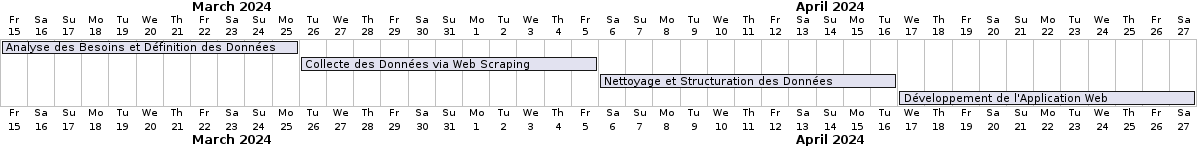
\includegraphics[width=\textwidth]{gantt1.png}
        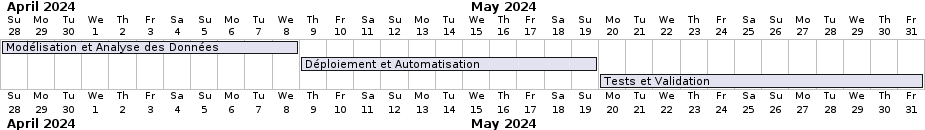
\includegraphics[width=\textwidth]{gantt2.png}
    \caption{Diagramme de Gantt}
\end{figure}



\newpage
%Chapter 3
\chapter{Le Web Scraping}
\section{Définition}
\vspace{0.5cm}
\large{
\par Le web scraping, également appelé extraction de données web, est une technique utilisée pour extraire des informations à partir de sites web. Cette méthode implique l'utilisation de logiciels ou de scripts pour parcourir et récupérer des données disponibles publiquement sur internet. Contrairement aux API, qui fournissent des données de manière structurée et contrôlée, le web scraping permet d'extraire des informations directement à partir des pages web, en imitant la navigation et l'interaction d'un utilisateur humain.\par
}
\section{Le Web Scraping dans notre Projet}
\vspace{0.5cm}
\large{
\par Dans le cadre de notre projet Simulateur de Calcul des Prix des Transactions Immobilières, le web scraping a été essentiel pour collecter les données nécessaires en raison du caractère privé des informations immobilières au Maroc. Nous avons ciblé les sites d'annonces immobilières, notamment avito.ma, pour extraire les données relatives aux biens immobiliers (appartements, maisons, villas, bureaux, locaux commerciaux) en fonction des villes et du type de transaction (vente ou location). Cette approche nous a permis de constituer une base de données riche et détaillée pour notre application.\par
}
\section{Benchmark des Outils de Scraping}
\vspace{0.5cm}
\large{
\par Pour réaliser le web scraping, plusieurs outils et frameworks sont disponibles. Nous avons effectué un benchmark des outils les plus populaires pour déterminer celui qui répondrait le mieux à nos besoins :\par
}
\vspace*{0.5cm}
\begin{enumerate}
    \item \large{\textbf{BeautifulSoup}: Une bibliothèque Python utilisée pour parser des documents HTML et XML. Elle est simple d'utilisation mais nécessite d'être combinée avec d'autres bibliothèques pour la gestion des requêtes HTTP. }
    \item \large{\textbf{Scrapy}: Un framework open-source en Python, spécialement conçu pour le web scraping. Il est très puissant et permet de gérer des projets de scraping complexes avec des fonctionnalités intégrées pour le crawling, le parsing, le stockage des données et la gestion des erreurs. }
    \item \large{\textbf{Selenium}: Un outil permettant d'automatiser les navigateurs web. Il est utile pour scraper des sites dynamiques générés par JavaScript, mais il est plus lent et plus lourd que les autres options.}
    \item \large{\textbf{Splash}: Un outil de rendu de pages web, capable d'exécuter JavaScript, qui peut être utilisé avec Scrapy pour scraper des sites dynamiques. Il offre une flexibilité pour gérer les pages complexes tout en restant intégré dans un environnement Scrapy.}
\end{enumerate}
\large{
\par Après avoir évalué ces options, nous avons opté pour Scrapy en combinaison avec Splash en raison de leur robustesse, de leur flexibilité et de leurs capacités avancées de gestion des projets de scraping.
}
\section{Méthodologie}
\large{
\par La méthodologie de web scraping que nous avons adoptée comprend les étapes suivantes :\par
}
\begin{enumerate}
    \item \textbf{Analyse des Sites Web Ciblés}
    \begin{itemize}
        \item[$\bullet$] Identification des sites web pertinents pour le projet.
        \item[$\bullet$] Analyse de la structure HTML des pages pour déterminer les éléments contenant les informations nécessaires (titres, prix, descriptions, localisations, etc.).
    \end{itemize}
    \item \textbf{Développement des Spiders}
    \begin{itemize}
        \item[$\bullet$] Création de spiders avec Scrapy pour automatiser la navigation et l'extraction des données.
        \item[$\bullet$] Intégration de Splash pour gérer les pages dynamiques et exécuter JavaScript.
        \item[$\bullet$] Implémentation de mécanismes pour contourner les blocages de bots, tels que l'utilisation de proxies et de délais aléatoires.
    \end{itemize}
    \item \textbf{Exécution et Collecte des Données}
    \begin{itemize}
        \item[$\bullet$] Exécution des spiders pour collecter les données brutes.
        \item[$\bullet$] Surveillance des performances et des erreurs lors de l'extraction.
    \end{itemize}
    \item \textbf{Nettoyage et Structuration des Données}
    \begin{itemize}
        \item[$\bullet$] Nettoyage des données pour éliminer les doublons, les annonces fausses et compléter les informations manquantes.
        \item[$\bullet$] Conversion et structuration des données pour les rendre utilisables dans notre application.
    \end{itemize}
    \item \textbf{Stockage des Données}
    \begin{itemize}
        \item[$\bullet$] Stockage des données collectées et nettoyées dans une base de données.
        \item[$\bullet$] Mise en place de procédures de sauvegarde et de gestion des données.
    \end{itemize}
\end{enumerate}
\large{
\par En suivant cette méthodologie, nous avons pu obtenir une base de données fiable et complète, essentielle pour le fonctionnement de notre simulateur de calcul des prix des transactions immobilières.\par
}

\newpage
\chapter{Analyse et Conception}
\section{Identification des Acteurs}
\vspace{0.5cm}
\begin{enumerate}
    \item \textbf{Utilisateurs Finaux}
    \begin{itemize}
        \item[$\bullet$] \textbf{Clients Gratuits}: Utilisateurs qui accèdent aux fonctionnalités de base pour effectuer des estimations simples et recevoir des notifications par défaut.
        \item[$\bullet$] \textbf{Clients Abonnés}: Utilisateurs payants ayant accès à des fonctionnalités avancées, incluant des estimations complexes, des notifications personnalisées, et des graphiques d'évolution des prix.
    \end{itemize}
    \item \textbf{Administrateurs}
    \begin{itemize}
        \item[$\bullet$] \textbf{Admin}: Utilisateurs responsables de la gestion et de la surveillance de l'application, y compris la gestion des utilisateurs, le contrôle de la fréquence de scraping .
    \end{itemize}
\end{enumerate}

\section{Besoins Fonctionnels}
\vspace{0.5cm}
\begin{enumerate}
    \item \textbf{Estimation de Prix}
    \begin{itemize}
        \item[$\bullet$] Permettre aux utilisateurs de saisir les caractéristiques d'un bien immobilier (type de bien, localisation, surface, nombre de pièces, etc.).
        \item[$\bullet$] Générer des estimations de prix de vente ou de location basées sur les données collectées et nettoyées.
    \end{itemize}
    \newpage
    \item \textbf{Notifications}
    \begin{itemize}
        \item[$\bullet$] Envoyer des notifications aux utilisateurs concernant les évolutions de prix des biens immobiliers similaires.
        \item[$\bullet$] Permettre aux utilisateurs abonnés de personnaliser leurs notifications selon leurs préférences.
    \end{itemize}
    \item \textbf{Tableau de Bord}
    \begin{itemize}
        \item[$\bullet$] Offrir un tableau de bord interactif pour les utilisateurs abonnés, affichant des graphiques et des indicateurs sur les tendances des prix.
        \item[$\bullet$] Fournir un tableau de bord administratif pour surveiller la performance du système, gérer les utilisateurs, et configurer la fréquence de scraping.
    \end{itemize}
    \item \textbf{Gestion des Utilisateurs}
    \begin{itemize}
        \item[$\bullet$] Permettre l'inscription et la gestion des comptes utilisateurs.
        \item[$\bullet$] Gérer les plans d'abonnement et les paiements .
    \end{itemize}
    \item \textbf{Automatisation }
    \begin{itemize}
        \item[$\bullet$] Automatiser le processus de scraping et de nettoyage des données.
    \end{itemize}
\end{enumerate}

\section{Besoins Non Fonctionnels}
\vspace{0.5cm}
\begin{enumerate}
    \item \textbf{Sécurité}
    \begin{itemize}
        \item[$\bullet$] Garantir la sécurité des données des utilisateurs, y compris la protection des informations personnelles et des données de paiement.
    \end{itemize}
    \item \textbf{Scalabilité}
    \begin{itemize}
        \item[$\bullet$] Concevoir l'application de manière à pouvoir évoluer pour gérer une augmentation du nombre d'utilisateurs et de données à traiter.
    \end{itemize}
    \item \textbf{Maintenance}
    \begin{itemize}
        \item[$\bullet$] Faciliter la maintenance et les mises à jour de l'application, avec une documentation complète et des procédures de sauvegarde régulières.
    \end{itemize}
\end{enumerate}

\newpage
\section{Diagramme de cas d'utilsation}
\vspace{0.5cm}
\begin{figure}[h]
    \centering
        
\includegraphics[width=\textwidth]{uml-client_gratuit.png}
    \caption{Diagramme de cas d'utilsation "Client Gratuit"}
\end{figure}
\newpage
\vspace*{3.5cm}
\begin{figure}[h]
    \centering
        
\includegraphics[width=\textwidth]{uml-Client_abonne.png}
    \caption{Diagramme de cas d'utilsation "Client Abonné"}
\end{figure}
\newpage
\vspace*{3.5cm}
\begin{figure}[h]
    \centering
        
\includegraphics[width=\textwidth]{uml-Admin.png}
    \caption{Diagramme de cas d'utilsation "Admin"}
\end{figure}

\newpage

\section{Diagramme d'activités}
\vspace{0.5cm}
\section{Diagramme de classes}
\vspace{0.5cm}
 





\end{document}